%%%%%%%%%%%%%%%%%%%%%%%%%%%%%%%%%%%%%%%%%%%%%%%%%%%%%%%%%%%%%%%%%%%%
\section{Integration and Installation (7 pages)}
\label{sec:fdsp-apa-install}

In this section, the full installation sequence will be detailed, from the arrival of the APAs at the Integration Facility (IF) all the way to the final positioning and integration inside the cryostat. 

After APAs have left the production site, they will be shipped to the IF for integration with the remaining systems (electronics for sure, maybe photon detectors if not integrated already at the production site). Different tests will be performed there to ensure the functioning of the fully integrated APAs. Once all the tests are satisfactory (we need a description of what happens when test failed), the APA is re-packaged to be sent to Homestake and underground. The APA crates are loaded in the cage by the sling and are lowered down to the underground location where they will be picked up and stored in the waiting area. They then will be removed from the crate, lowered in the TOC, where cables will be installed (if not already all installed at the IF) and final tests will be performed once the APAs are in place (exact tests need to be finalized. Do we do tests near the TCO in case of problems, or we install a full "wall ACACA" before testing the wall at once).

%%%%%%%%%%%%%%%%%%%%%%%%%%%%%%%%%%%
\subsection{Transport and Handling}
\label{sec:fdsp-apa-install-transport}

This section will describe the crates used for transport of the APA (both for international shipping and for shipping between IF and underground, which may be different). The APA frame feature for handling should have been described in section \ref{sec:fdsp-apa-boards}, where it says anchoring). The APA will have been inserted in the crate at the production site and shipped to the IF.

A description of the handling at IF is required. We need cranes to get the APAs out of the crate and moved them to a temporary holder for integration and testing. Once this is completed, the APA will be moved back to the crate (or to different crates) for the transport underground. These crates will be loaded on a truck, driven to the mine, transported to the cage, secured on the sling under the cage, lowered down, picked up (probably rotation of 180$^{\circ}$) and moved to the underground storage area. There, they will be lifted out of the crate and moved down the TCO. Once final tests have been performed, the APAs will be moved to their final location.

List of figures will be:
\begin{itemize}

\item{Drawing of the crates for shipping (two different if required)}
\item{Drawing of the IF holder for the APA integration and testing}
\item{Drawing of the way APA crates will be attached under the cage}
\item{Drawing of the storage area and the cranes and holder for APAs}
\item{Drawing of the system to move the APAs down the TCO and inside the cryostat}

\end{itemize}

%%%%%%%%%%%%%%%%%%%%%%%%%%%%%%%%%%%
\subsection{Integration with Photon Detectors and TPC Electronics}
\label{sec:fdsp-apa-install-pds-elec}

For the photon detector system (PDS): The current idea is to integrate them at the production sites. This is clearly the easiest since the frames are available with no wires. However, it is possible that this will need to be done at the IF. Detailed plans of the PDS integration are required.  

List of figures for the PDS will be:
\begin{itemize}
\item{Drawing of the PDS system installed on the APA}
\item{Potential drawings of the sequence of PDS installation and connections}
\end{itemize}

For the electronics: The electronics will be connected to the APAs at the IF. A detailed description of the sequence of installation should be here.

List of figures for the electronics will be:
\begin{itemize}
\item{Drawing of the electronics installed on the APA}
\item{Potential drawings of the sequence of electronics installation and connections}
\end{itemize}


%%%%%%%%%%%%%%%%%%%%%%%%%%%%%%%%%%%
\subsection{Installation in the cryostat}
\label{sec:fdsp-apa-install-cryostat}

A detailed description of the installation sequence once the APAs are underground is required. After the APA is out of the crate and supported, test describe in ref{sec:fdsp-apa-install-calib} will be performed. Then the APA is lowered down in the TCO. Some cables will likely need to be installed here, and the APA will be secured inside the cryostat, while the second APA will be lowered in the TCO. The two APAs will need final cabling and connection between the two. May be some quick testing before the two linked APAs are moved to final location.

List of figures for the installation in the cryostat will be:
\begin{itemize}
\item{Drawing of the sequence from the underground storage to TCO}
\item{Drawing of the cable installation required}
\item{Drawing of the link/connection between the two APAs}
\end{itemize}

%%%%%%%%%%%%%%%%%%%%%%%%%%%%%%%%%%%
\subsection{Quality Control in Integration and Installation}
\label{sec:fdsp-apa-install-calib}

This section will describe all the tests that will be performed to ensure that each APA is fully functional and to the specifications required. There will be two main testing step. One at the Integration Facility and one once the APA are installed into their location in the cryostat.

A quality control dedicated database is required to keep track of all the different channels in all the different APAs at the different stages of the installation and integration. A simple and practical method of tagging critical parts in the APA will also be essential for efficient integration.


\subsubsection{Quality Control at Integration Facility}

All the active detector components will be shipped to the Integration Facility for integration between the different parts and for testing. It is at that location that we will have most time to perform tests and this step will be critical for ensuring high performance of the integrated APAs. The exact time scale of the APAs still needs to be finlaised based on information from the production sites and on installation schedule.

Table \ref{tab:qclist} shows a summary of all the quality control tests that will be performed at the IF. The details of each is given below. Figure \ref{fig:testlayout} shows an example of the layout of the testing area at the IF.

\begin{dunetable}[QC List]{l|c|c}{tab:qclist}{qclist}   
Test to perform   &  Number of wires/channels & Acceptable values\\ 
Visual Inspection & All & All intact\\
Wire tension      & XX$\%$ sample & 5 $\pm$ 1N\\
Wire continuity   & All & $-$\\
Electronics connections & All & Perfect\\
Noise             & All &  $\pm$ XX\\
Cold test         & All & All intact\\
\end{dunetable}

\begin{dunefigure}[Schematics of the layout of the IF testing area]{fig:testlayout}{A schematic of the layout for the testing area at the IF. Most of this area has to be embedded in a clean environment (i.e. tent).}
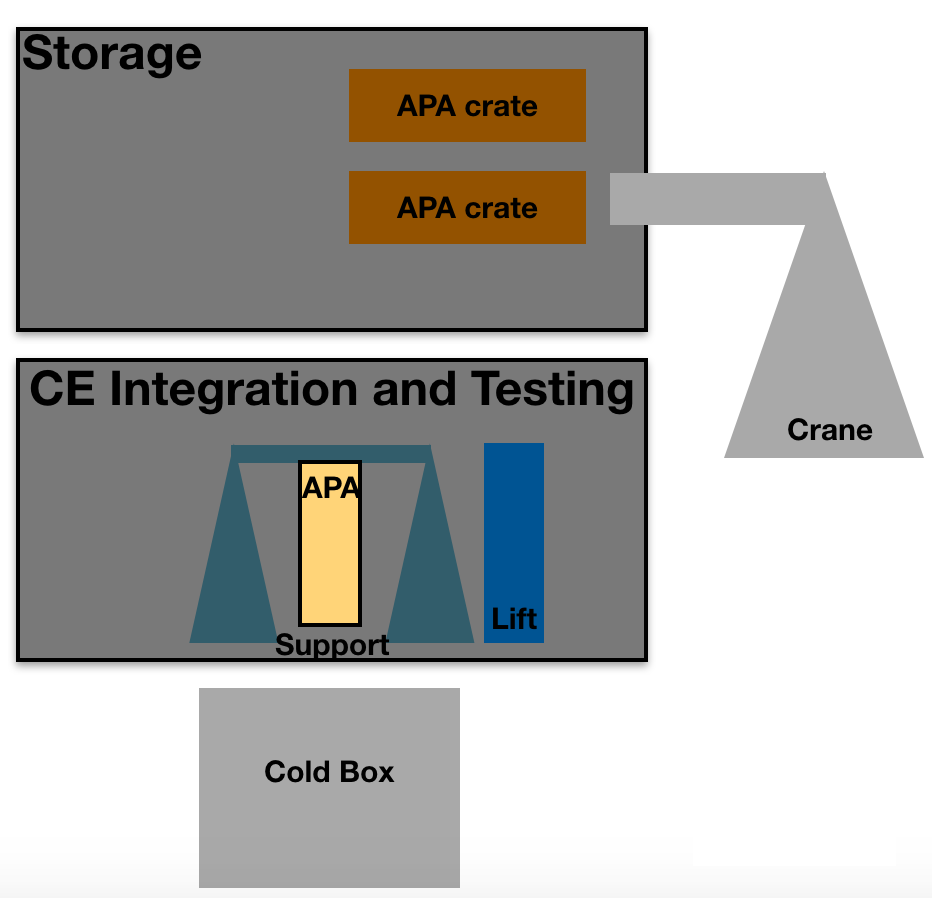
\includegraphics[width=0.5\textwidth]{test_layout.png} 
\end{dunefigure}

After unpacking an APA, a thorough visual inspection will be performed. A sample of around xxx wires (representing about xx$\%$ of the wires) will be  measured for tension. Tension measurements will be performed following the laser method (same as protoDUNE). However, alternative methods, using voltage measurements are also being pursued to reduce the measuring time, which is currently a significant time driver. The values will be recorded in the database and compared with the full-scale original tension measurement. Definite guidance for the acceptable tension values will be available to inform decision on the quality of the APA. A clear pass/fail criteria will be provided as well as a clear procedures to deal with individual wires laying outside the acceptable values. A continuity test will be performed on all the wires and the data will be recorded. Note that the requirement for a successfully quality controlled APA is where \textbf{less than $1\%$ of the channels are broken or dead}. Exact relation between lower or higher tension and the acceptance of a channel still needs to be worked out.

Once the electronics is installed by the Electronics consortium, serious testing of the APA readout should be performed. The integrated APA should be inserted in the cold box and the electronics performance (signal, noise,...) can be tested adequately. A strict guidance will be available to assess the pass/fail criteria for each APA during these tests.

When all the tests have been successfully performed, the APA will be tagged as good and will be prepared for shipping to SURF.

\subsubsection{Quality Control underground}

There are three opportunities to test the APAs underground. In the storage area, once secured in the TCO or once positioned at their final location. The latter is probably the most important and it might be good to save time to perform the final tests once the full "ACACA wall". This brings the risk that if serious problems are found, they are harder (more time consuming) to move out. Both in the TCO and final location is the only way we can test the fully connected APA, therefore tests here are absolutely required. 

\subsubsection{Tests underground in the storage/unpacking area}

The APAs will be unpacked in the storage area underground (see Figure~\ref{fig:storage}). Space in this area is very limited and only visual inspection will be performed during unpacking. If clear defects are visible, the APA will be return to the IF for further investigation.

\begin{dunefigure}[Schematics of the underground layout in the storage area]{fig:storage}{A schematic of the layout for the storage and unpacking area underground.}
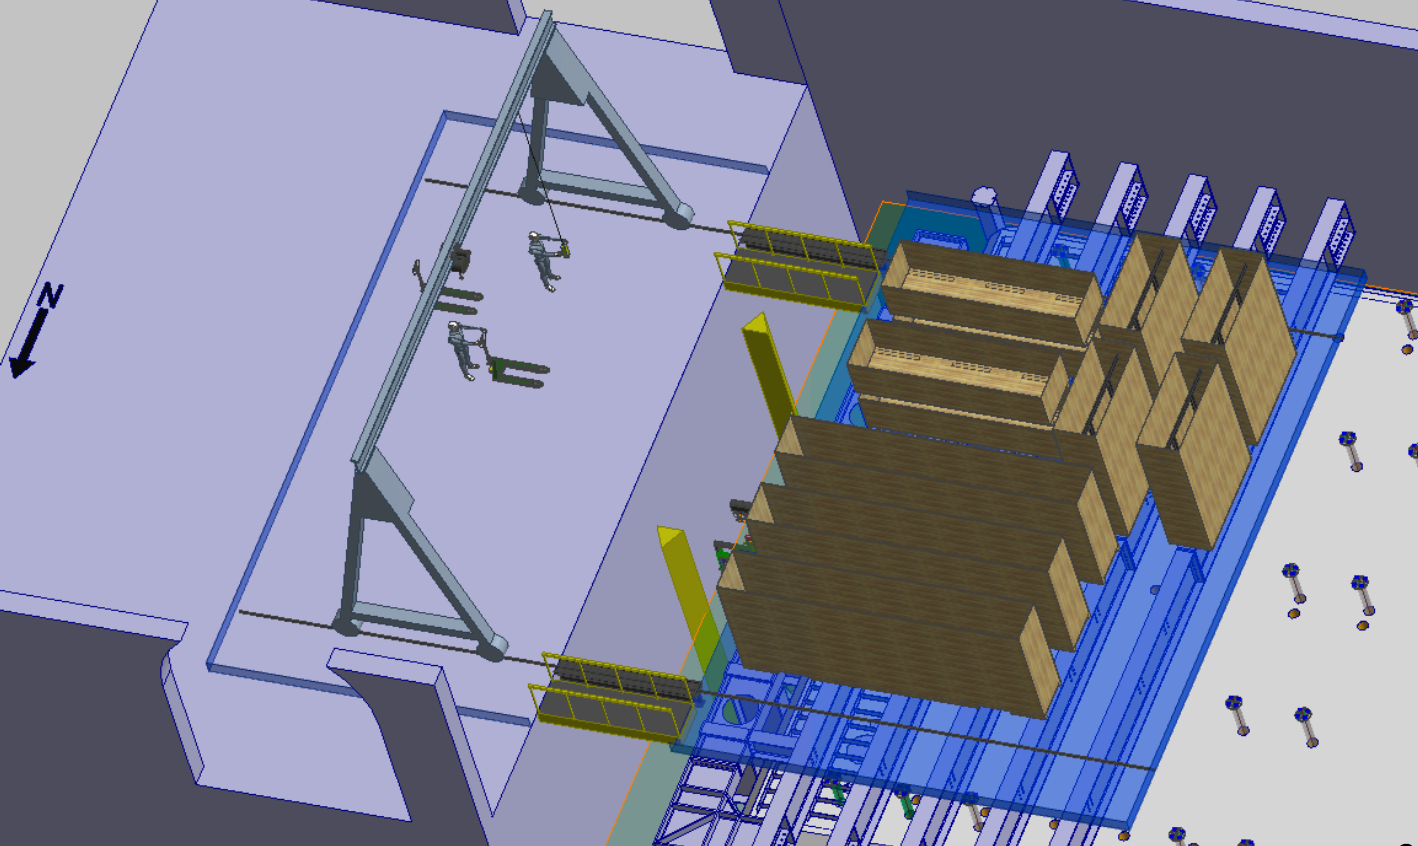
\includegraphics[width=0.5\textwidth]{storage.png} 
\end{dunefigure}

\subsubsection{Tests underground in the TCO area}

Pairs of APA (top and bottom) will be lowered in the TCO to be linked and cabled. Once the cabling is finished a connection test will need to be performed to ensure adequate cabling. Due to the very restrictive space in the TCO (see Figure~\ref{fig:tco}, no additional tests then visual inspection will be performed at that time and the cabled and linked APAs will be positioned in their final location in the cryostat.

\begin{dunefigure}[Schematics of the TCO  area]{fig:tco}{A schematic of the layout for the TCO area underground.}
\begin{tabular}{cc}
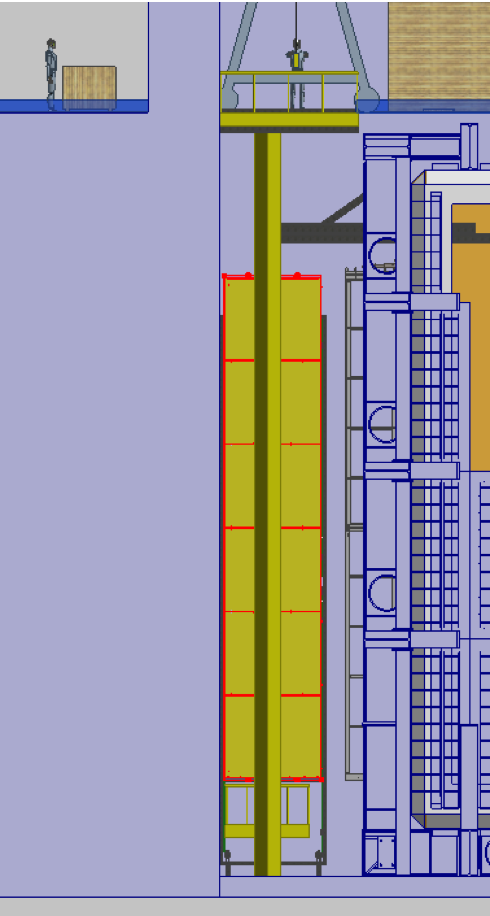
\includegraphics[width=0.23\textwidth]{tco1.png} &
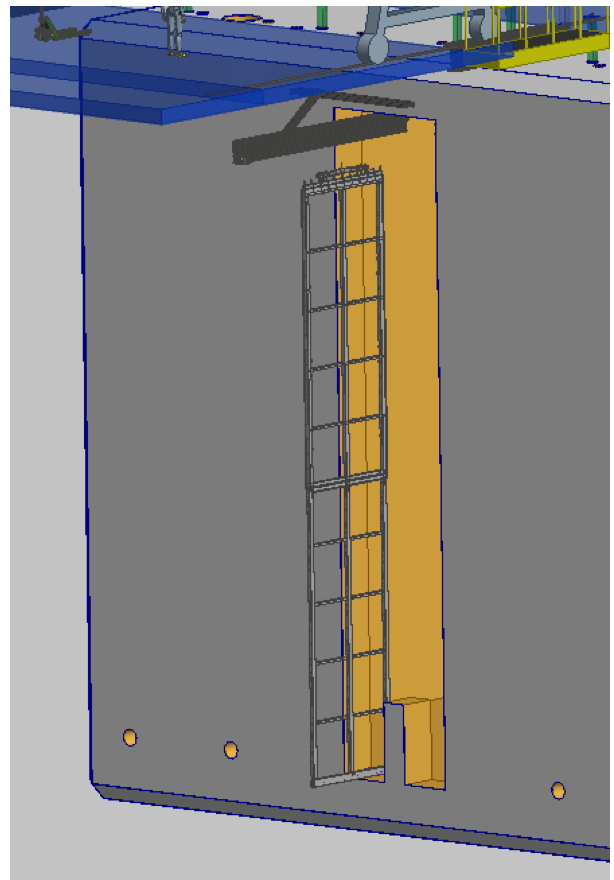
\includegraphics[width=0.3\textwidth]{tco2.png}
\end{tabular}
\end{dunefigure}

\subsubsection{Tests underground in the cryostat}

The current goal is to install a full APA-CPA-APA-CPA-APA wall every week (see Figure~\ref{fig:wall}. After each wall is installed, the night crew will have time for final testing of the installed APA. There are currently two testing models, one where the night crew will test APA pairs as they are installed (every two days), and the other model where the night crew will test the full wall at once. The decision between the two models will be made when accurate estimates of the time needed for the testing will be available.

\begin{dunefigure}[Schematics of the wall in the cryostat]{fig:wall}{A schematic of the layout of a full APA-CPA-APA-CPA-APA wall installed in the cryostat.}
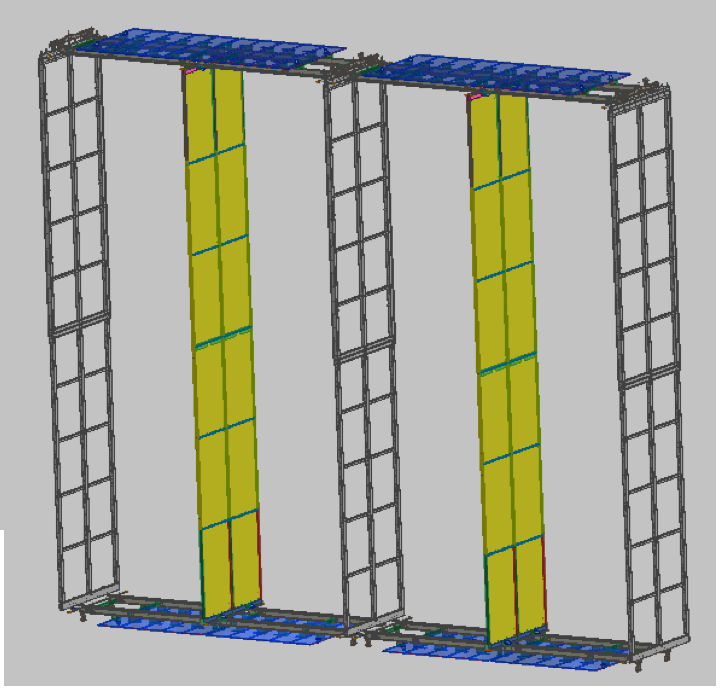
\includegraphics[width=0.5\textwidth]{wall.png}
\end{dunefigure}

The tests performed will be the same described above at the IF. Tension on a smaller set of wires will be measured to ensure that the installation operations did not alter the APAs. Since the full integration is now done, a full readout test can be performed. Short runs will be taken with the DAQ system to ensure that the full readout is fully operational. The details of these tests still need to be developed to allow efficient assessment of the integrated APAs.

\subsubsection{Summary of the QC protocols}

In order to ensure fully operational APAs in the far detector, a series of tests has been developed along the APA installation steps. Major testing will be performed at the Integration Facility, visual inspection will be done at every steps of APA handling (in the underground storage area after unpacking and in the TCO after lowering). Some minimal testing will be performed in the TCO after APA pairs are linked and cabled and finally an final extensive testing campaign will be performed in the fully integrated APAs once positioned at their final location in the cryostat. At each of these testing steps, the requirement of less than $1\%$ of dead or unresponsive channels will be respected.

